\documentclass{article}

\usepackage{graphicx}
\usepackage{tikz}
\usepackage{tikzsymbols}
\usetikzlibrary{calc,patterns,shapes.geometric}
\pagestyle{empty}
\usepackage[margin=0pt]{geometry}
\geometry{papersize={14in,12in}}

\def\centerarc[#1](#2)(#3:#4:#5){\draw[#1] ($(#2)+({#5*cos(#3)},{#5*sin(#3)})$) arc (#3:#4:#5);}

\begin{document}
	\begin{figure}
		\centering
		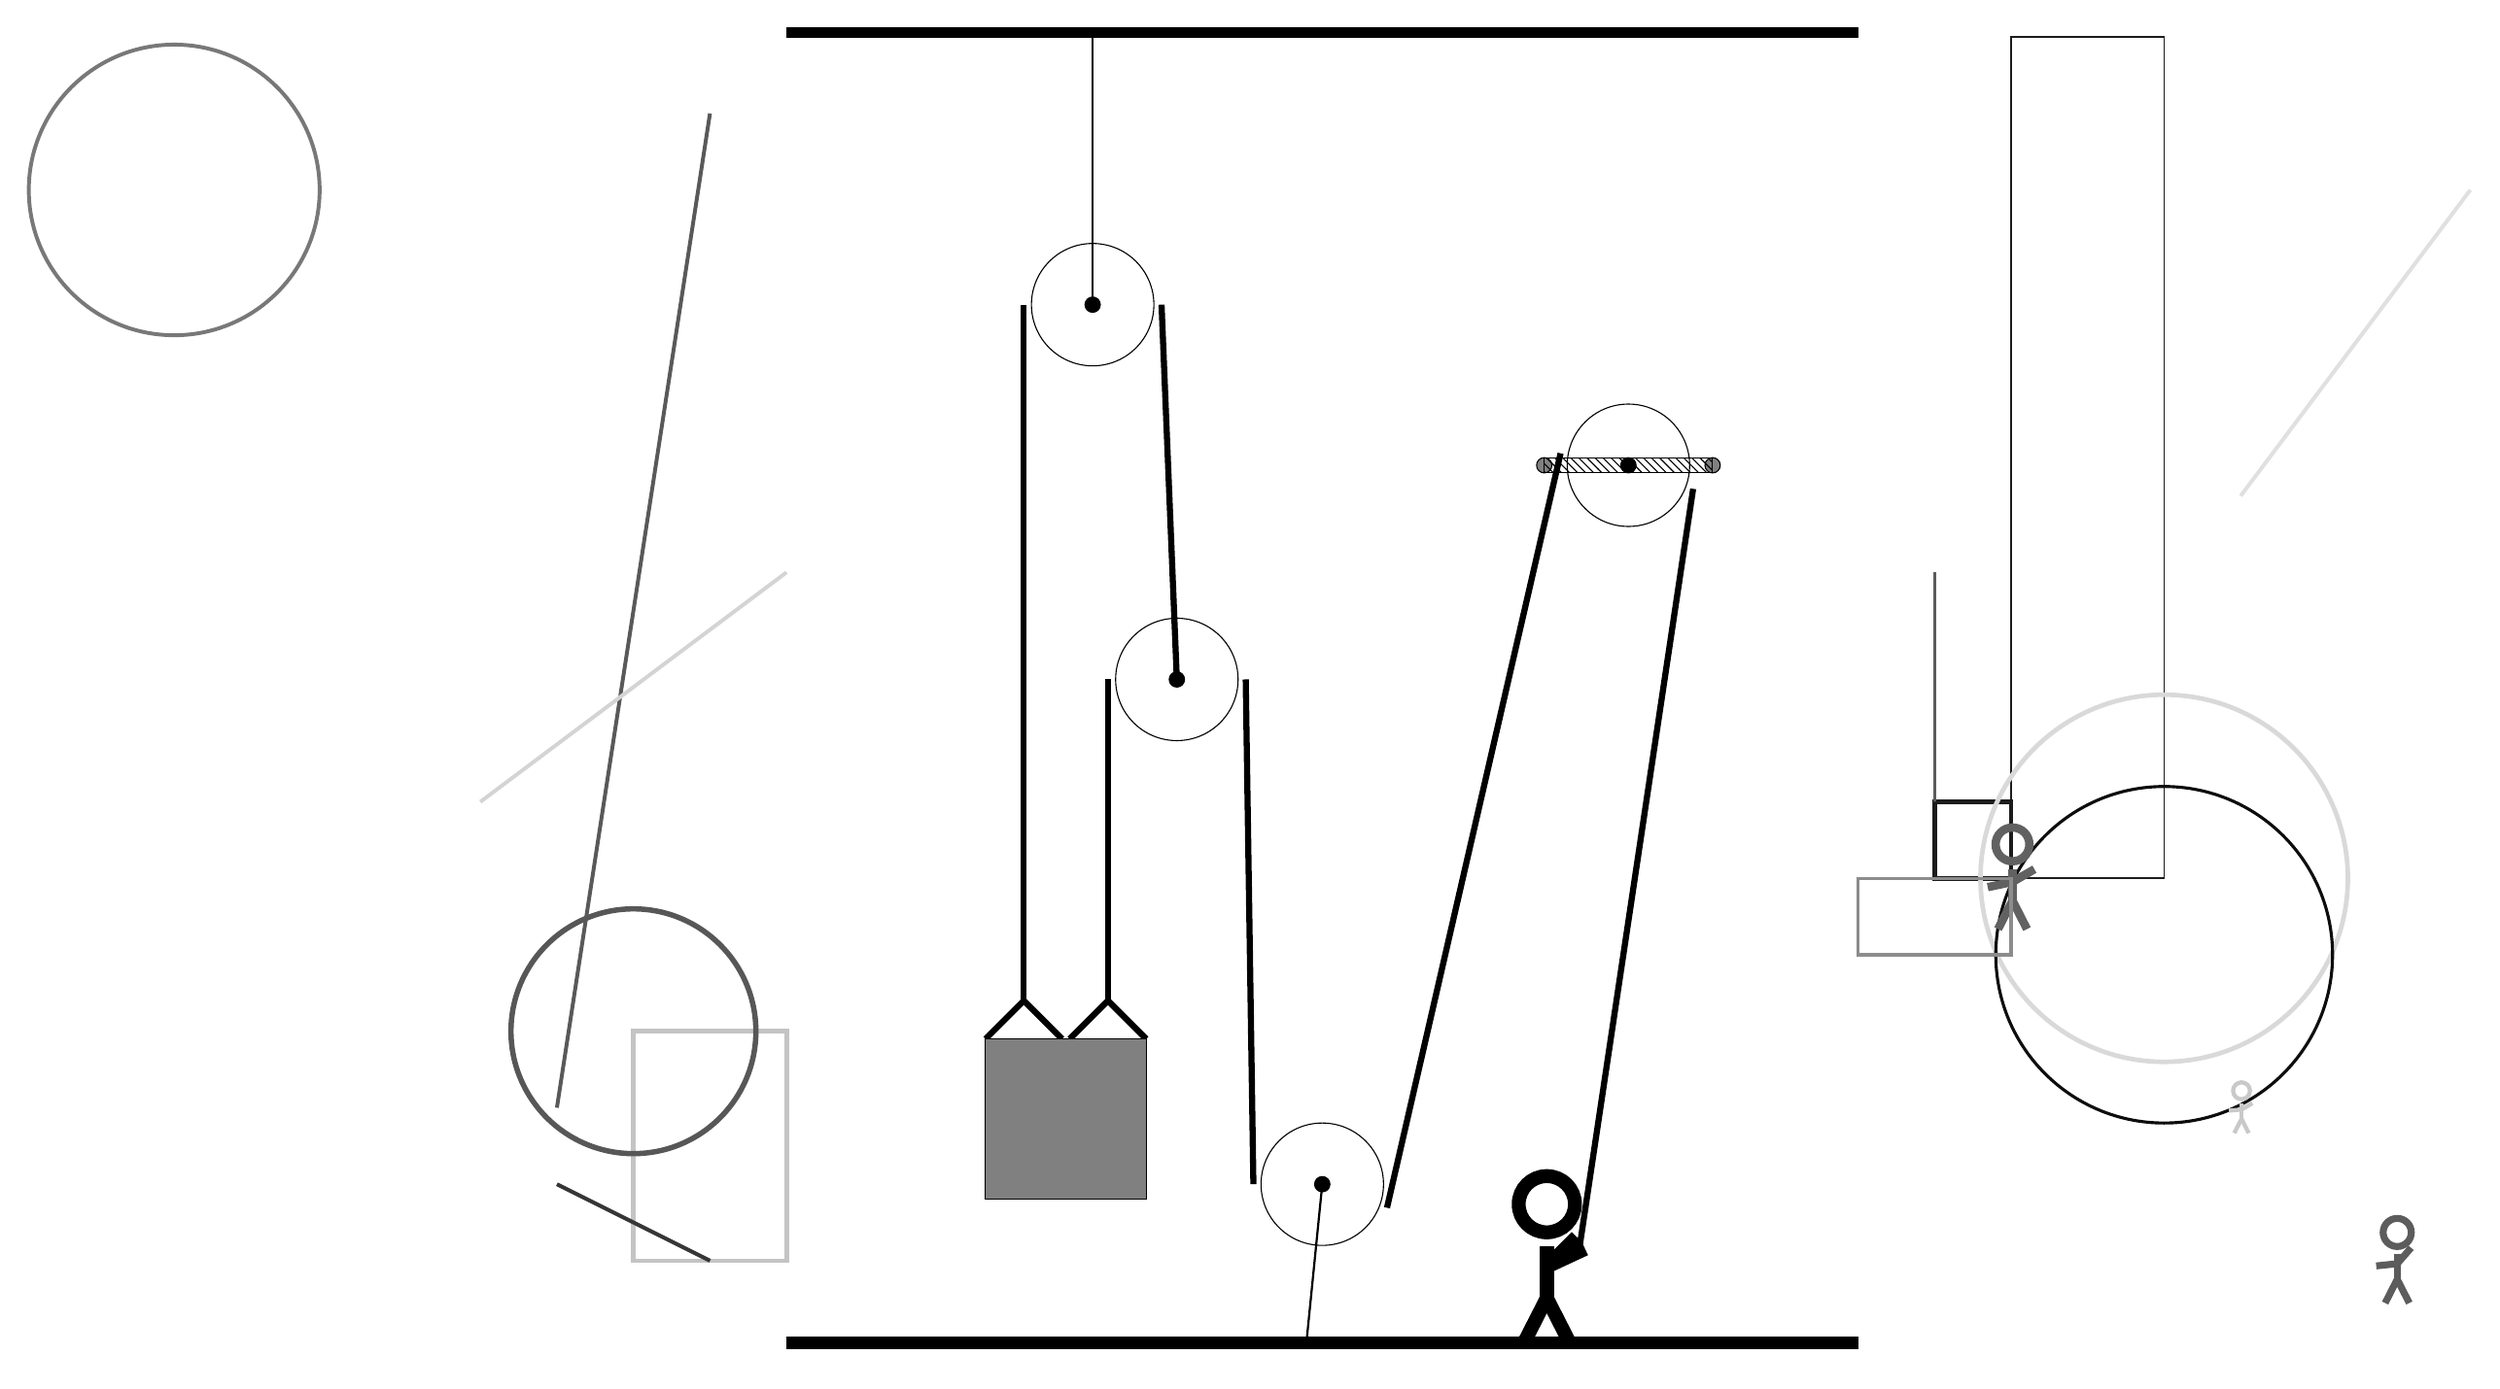
\begin{tikzpicture}
			%%%%% START %%%%%
			
			\draw[fill=black] (-2, 14) rectangle (12, 14.125);
			
			\draw[line width=0.2mm, color=black!89] (14, 14) rectangle (16, 3);
			
			\draw[line width=0.6mm, color=black!89] (14, 4) rectangle (13, 3);
			\draw [line width=0.5mm, color=black!53](-10, 12) circle (1.9);
			\draw[line width=0.6mm, color=black!23] (-4, 1) rectangle (-2, -2);
			\draw [line width=0.6mm, color=black!15](16, 3) circle (2.4);
			
			\draw[line width=0.5mm, color=black!79](-3, -2) -- (-5, -1);
			\draw [line width=0.4mm, color=black!95](16, 2) circle (2.2);
			\node[line width=0.7mm, color=black!62] at (14, 3) {\Strichmaxerl[6][12][30]};
			\draw[line width=0.4mm, color=black!64] (13, 7) rectangle (13, 4);
			\node[line width=0.3mm, color=black!64] at (19, -2) {\Strichmaxerl[5][6][49]};
			\draw[line width=0.5mm, color=black!12](17, 8) -- (20, 12);
			\draw[line width=0.4mm, color=black!45] (14, 3) rectangle (12, 2);
			\node[line width=0.5mm, color=black!21] at (17, 0) {\Strichmaxerl[3][5][30]};
			\draw[line width=0.5mm, color=black!65](-5, 0) -- (-3, 13);
			\draw[line width=0.5mm, color=black!17](-6, 4) -- (-2, 7);
			\draw [line width=0.7mm, color=black!66](-4, 1) circle (1.6);
			
			\draw (2, 10.5) circle (0.8);
			\draw[fill=black] (2, 10.5) circle (0.1);
			\draw[thick] (2, 10.5) -- (2, 14);
			
			\draw (3.1, 5.6) circle (0.8);
			\draw[fill=black] (3.1, 5.6) circle (0.1);
			
			\draw (5, -1) circle (0.8);
			\draw[fill=black] (5, -1) circle (0.1);
			\draw[thick] (5, -1) -- (4.8, -3);
			
			\draw (9, 8.4) circle (0.8);
			\draw[fill=black] (9, 8.4) circle (0.1);
			\draw[fill=black!50] (7.9, 8.4) circle (0.1);
			\draw[fill=black!50] (10.1, 8.4) circle (0.1);
			\draw[pattern=north west lines, pattern color=black] (7.9, 8.5) rectangle (10.1, 8.3);
			
			\draw[line width = 0.8mm]  (0.6, 0.9) -- (1.1, 1.4) -- (1.6, 0.9);
			\draw[line width = 0.8mm]  (1.7, 0.9) -- (2.2, 1.4) -- (2.7, 0.9);
			\draw[fill=black!50] (0.6, 0.9) rectangle (2.7, -1.2);
			
			\draw[line width = 0.8mm] (1.1, 10.5) -- (1.1, 1.4);
			\centerarc[line width = 0.8mm](2, 10.5)(0:180:0.9);
			\draw[line width = 0.8mm] (2.9, 10.5) -- (3.1, 5.6);
			\draw[line width = 0.8mm] (2.2, 5.6) -- (2.2, 1.4);
			\centerarc[line width = 0.8mm](3.1, 5.6)(0:180:0.9);
			\draw[line width = 0.8mm] (4.0, 5.6) -- (4.1, -1);
			\centerarc[line width = 0.8mm](5, -1)(180:340:0.9);
			\draw[line width=0.8mm](5.8457, -1.3078) -- (8.1137, 8.5562);
			\centerarc[line width = 0.8mm](9, 8.4)(-20:170:0.9);
			\draw[line width=0.8mm](9.8457, 8.0922) --  (8.35, -1.9);
			
			\node at (8, -2) {\Strichmaxerl[10][225][25]};
			
			\draw[fill=black] (-2, -3) rectangle (12, -3.15);
			
			%%%%% END %%%%%
		\end{tikzpicture}
	\end{figure}	
\end{document}